\documentclass[usenames,dvipsnames,t]{beamer}
\usetheme{Frankfurt}

\usepackage{tikz}
\usepackage[utf8]{inputenc}
\usepackage{setspace}
\usepackage{bbding}
\usepackage{microtype}

\setbeamertemplate{navigation symbols}{}

\title{Implementing Genesis \\ \emph{\normalsize Completely Revised Second Edition}}
\author{Edsko de Vries}
\institute{Well-Typed}
\date{Feb 18, 2021}

\begin{document}

\frame{\titlepage}

%%%%%%%%%%%%%%%%%%%%%%%%%%%%%%%%%%%%%%%%%%%%%%%%%%%%%%%%%%%%%%%%%%%%%%%%%%%%%%%%

\begin{frame}
\frametitle{Chain selection rule}

\begin{alertblock}{Density rule}
A candidate chain is preferred over our current chain if it is denser
(contains more blocks) in a window of $s$ slots anchored at the intersection
between the two chains.
\end{alertblock}

\pause

\begin{alertblock}{Genesis window size}
The genesis window size $s$ will be set to $s = 3k/f$.
\end{alertblock}

\end{frame}

%%%%%%%%%%%%%%%%%%%%%%%%%%%%%%%%%%%%%%%%%%%%%%%%%%%%%%%%%%%%%%%%%%%%%%%%%%%%%%%%

% TODO: Maybe discuss rule equivalence?

%%%%%%%%%%%%%%%%%%%%%%%%%%%%%%%%%%%%%%%%%%%%%%%%%%%%%%%%%%%%%%%%%%%%%%%%%%%%%%%%

\begin{frame}
\frametitle{Fragment selection}

\begin{center}
\begin{tikzpicture}[yscale=0.7]
\draw (0,0) -- ++( 1,  0) coordinate(b1);
\draw (b1)  -- ++( 1,  1) coordinate(b2);
\draw (b2)  -- ++( 1,  1) -- ++(2  , 0) node[right=1.5cm]{a};
\draw (b2)  -- ++( 1, -1) -- ++(1  , 0) coordinate(b3);
\draw (b3)  -- ++( 1,  1) -- ++(1.5, 0) node[right]{b};
\draw (b3)  -- ++( 1, -1) -- ++(0.5, 0) node[right=1cm]{c};
\draw (b1)  -- ++( 2, -2) -- ++(3  , 0) node[right=0.5cm]{d};
%
\path % adjust bounding box
     (3.5,2.5)
  -- (3.5,1.5)
  -- (2, 0)
  -- (3.5, -1.25)
  -- (3.5, -2.5);
\end{tikzpicture}
\end{center}

\end{frame}

%%%%%%%%%%%%%%%%%%%%%%%%%%%%%%%%%%%%%%%%%%%%%%%%%%%%%%%%%%%%%%%%%%%%%%%%%%%%%%%%

\begin{frame}
\frametitle{Fragment selection}

\begin{center}
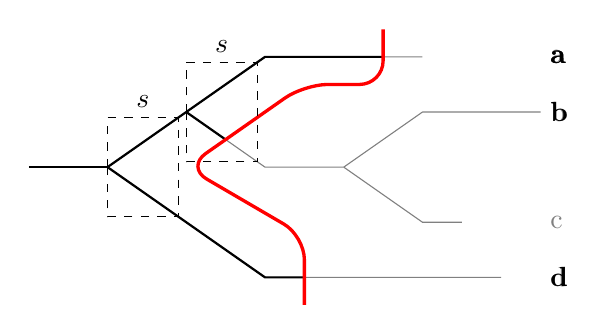
\begin{tikzpicture}[yscale=0.7]
\draw [thin, gray] (0,0) -- ++( 1,  0) coordinate(b1);
\draw [thin, gray] (b1)  -- ++( 1,  1) coordinate(b2);
\draw [thin, gray] (b2)  -- ++( 1,  1) -- ++(2  , 0) coordinate(a) node[right=1.5cm]{a};
\draw [thin, gray] (b2)  -- ++( 1, -1) -- ++(1  , 0) coordinate(b3);
\draw [thin, gray] (b3)  -- ++( 1,  1) -- ++(1.5, 0) coordinate(b) node[right]{b};
\draw [thin, gray] (b3)  -- ++( 1, -1) -- ++(0.5, 0) node[right=1cm]{c};
\draw [thin, gray] (b1)  -- ++( 2, -2) -- ++(3  , 0) coordinate(d) node[right=0.5cm]{d};
%
\draw [thick] (0,0) -- ++( 1,  0);
\draw [thick] (b1)  -- ++( 1,  1);
\draw [thick] (b2)  -- ++( 1,  1) -- ++(1.5, 0);
\draw [thick] (b2)  -- ++(0.5, -0.5);
\draw [thick] (b1)  -- ++( 2, -2) -- ++(0.5, 0);
%
\draw[very thick, rounded corners=3mm, red]
     (4.5,2.5)
  -- (4.5,1.5)
  -- (3.5,1.5)
  -- (2, 0)
  -- (3.5, -1.25)
  -- (3.5, -2.5);

\onslide<3>{
  \draw [dashed]
       (b1)
    -- ++(   0,  0.9)
    -- ++( 0.9,  0  ) node[pos=0.5,above]{$s$}
    -- ++(   0, -1.8)
    -- ++(-0.9,  0  )
    -- cycle;
  \node at (a) [right=1.5cm] {\textbf{a}};
  \node at (d) [right=0.5cm] {\textbf{d}};
}

\onslide<4>{
  \draw [dashed]
       (b2)
    -- ++(   0,  0.9)
    -- ++( 0.9,  0  ) node[pos=0.5,above]{$s$}
    -- ++(   0, -1.8)
    -- ++(-0.9,  0  )
    -- cycle;
  \node at (a) [right=1.5cm] {\textbf{a}};
  \node at (b) [right] {\textbf{b}};
}

\end{tikzpicture}
\end{center}

\onslide<2->{
\begin{alertblock}{Fragment selection}
Let $\mathcal{S}$ be set of chain fragments, all anchored at the same point
(that is, the fragments share a common ancestor), corresponding to some set of
chains $\mathcal{C}$. Then $A$ is a preferred fragment in $\mathcal{S}$ if and
only if $A$ is a fragment of a preferred chain in $\mathcal{C}$.
\end{alertblock}
}

\end{frame}

%%%%%%%%%%%%%%%%%%%%%%%%%%%%%%%%%%%%%%%%%%%%%%%%%%%%%%%%%%%%%%%%%%%%%%%%%%%%%%%%

\begin{frame}{Known density}

We say that a chain fragment has a \emph{known density} at some point $p$
if either of the following conditions hold:

\begin{enumerate}
\item The fragment contains a block after at least $s$ slots:
\begin{center}
\begin{tikzpicture}[yscale=0.75]
\path (0,0) -- (9,0); % adjust bounding box
\path (0,0) -- (1,0) node[pos=0.5]{$\cdots$};
\draw
     (1,0)
  -- (3,0)   node{$\bullet$} node[above left]{$p$} coordinate(p)
  -- (3.5,0) node{$\bullet$}
  -- (4,0);
\path
     (4,0)
  -- (5,0) node[pos=0.5]{$\cdots$};
\draw
     (5,0)
  -- (5,0) node{$\bullet$}
  -- (6,0) node{$\bullet$}
  -- (7,0) node[red]{$\bullet$}
  -- (8,0) node[right]{$\cdots$};
\draw [dashed]
     (p)
  -- ++(0, 1)
  -- ++(3.5, 0) node[pos=0.5,above]{$s$ slots}
  -- ++(0, -2)
  -- ++(-3.5, 0)
  -- cycle;
\end{tikzpicture}
\end{center}

\item The chain (not just the fragment) terminates within the window:
\begin{center}
\begin{tikzpicture}[yscale=0.75]
\path (0,0) -- (9,0); % adjust bounding box
\path (0,0) -- (1,0) node[pos=0.5]{$\cdots$};
\draw
     (1,0)
  -- (3,0)   node{$\bullet$} node[above left]{$p$} coordinate(p)
  -- (3.5,0) node{$\bullet$}
  -- (4,0);
\path
     (4,0)
  -- (5,0) node[pos=0.5]{$\cdots$};
\draw
     (5,0)
  -- (6,0) node[red]{$\bullet$};
\draw [dashed]
     (p)
  -- ++(0, 1)
  -- ++(3.5, 0) node[pos=0.5,above]{$s$ slots}
  -- ++(0, -2)
  -- ++(-3.5, 0)
  -- cycle;
\end{tikzpicture}
\end{center}
\end{enumerate}

\end{frame}

%%%%%%%%%%%%%%%%%%%%%%%%%%%%%%%%%%%%%%%%%%%%%%%%%%%%%%%%%%%%%%%%%%%%%%%%%%%%%%%%

\begin{frame}{Fragment selection}

\begin{alertblock}{Look-ahead closure}
\label{lookahead-closure}
Let $\mathcal{S}$ be a set of chain fragments all anchored at the same point. We
say that $\mathcal{S}$ is \emph{look-ahead closed} if whenever there are two
fragments $A, B \in \mathcal{S}$, the densities of $A$ and $B$ are known at
their intersection.
\end{alertblock}

\pause

Unfortunately, requires unbounded lookahead:

\begin{center}
\begin{tikzpicture}[yscale=0.5]
\path (0,0) coordinate(I);
%
\node at (I) {$\bullet$};
\draw (I) -- ++(2.5, 0);
\draw (I) -- ++(1,-1) -- ++(0.5,0) coordinate(A) -- ++(2,0);
\draw [dashed]
     (I)
  -- ++(0,0.25)
  -- ++(2,0)
  -- ++(0,-1.5)
  -- ++(-2,0) node[pos=0.5,below]{$\underbrace{\hspace{2cm}}_\text{$s$ slots}$}
  -- cycle;
%
\node at (A) {$\bullet$};
\draw (A) -- ++(2.5, 0);
\draw (A) -- ++(1,-1) -- ++(0.5,0) coordinate(B) -- ++(2,0);
\draw [dashed]
     (A)
  -- ++(0,0.25)
  -- ++(2,0)
  -- ++(0,-1.5)
  -- ++(-2,0) node[pos=0.5,below]{$\underbrace{\hspace{2cm}}_\text{$s$ slots}$}
  -- cycle;
%
\node at (B) {$\bullet$};
\draw (B) -- ++(2.5, 0);
\draw (B) -- ++(1,-1) -- ++(0.5,0) coordinate(C) -- ++(2,0) node[above=0.5cm, right]{$\cdots$};
\draw [dashed]
     (B)
  -- ++(0,0.25)
  -- ++(2,0)
  -- ++(0,-1.5)
  -- ++(-2,0) node[pos=0.5,below]{$\underbrace{\hspace{2cm}}_\text{$s$ slots}$}
  -- cycle;
\end{tikzpicture}
\end{center}

\end{frame}

%%%%%%%%%%%%%%%%%%%%%%%%%%%%%%%%%%%%%%%%%%%%%%%%%%%%%%%%%%%%%%%%%%%%%%%%%%%%%%%%

\begin{frame}{Preferred Prefix}

\begin{equation*}
\mathcal{S} = \left\{ \;
\begin{tikzpicture}[baseline=0pt, xscale=0.5,yscale=0.5]
\draw [very thick, red] (-2,0) -- (0,0);
\draw (0,0) -- (1, 1) -- (6,  1) node[right]{$A$};
\draw (0,0) -- (1,-1) -- (7, -1) node[right]{$B$};
\draw [dashed] (-2,0) -- ++(0,1.5) -- ++(5,0) node[pos=0.5,above]{$\overbrace{\hspace{2cm}}^\text{$s$ slots}$} -- ++(0,-3) -- ++(-5,0) -- cycle;
\end{tikzpicture}
\right\}
\end{equation*}

\pause

\begin{alertblock}{Preferred prefix}
Given a set $\mathcal{S}$ of chain fragments, all anchored at the same point, a
preferred prefix is a prefix $\Pi$ of one of the fragments in $\mathcal{S}$,
such that $\Pi$ is guaranteed to be a prefix of a preferred fragment in the
lookahead-closure of $\mathcal{S}$.
\end{alertblock}

\end{frame}

%%%%%%%%%%%%%%%%%%%%%%%%%%%%%%%%%%%%%%%%%%%%%%%%%%%%%%%%%%%%%%%%%%%%%%%%%%%%%%%%

\begin{frame}{Prefix selection}

\begin{alertblock}{Step 1: Resolve initial fork}
\begin{center}
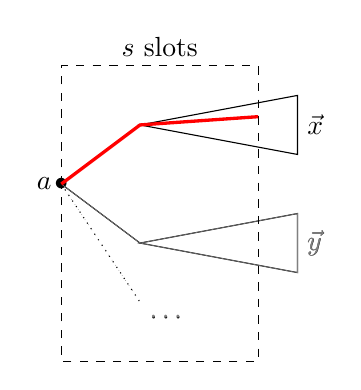
\begin{tikzpicture}[yscale=1.5]
\node at (0,0) [left] {$a$};
\node at (0,0) {$\bullet$};
%
\draw (0,0) -- (1, 0.5) coordinate(x);
%
\draw (x) -- ++(2,  0.25) -- ++(0, -0.5) node[pos=0.5,right]{$\vec{x}$} -- cycle;
\onslide<1>{
  \draw (0,0) -- (1,-0.5) coordinate(y);
  \draw (y) -- ++(2,  0.25) -- ++(0, -0.5) node[pos=0.5,right]{$\vec{y}$} -- cycle;
  \draw [dotted] (0,0) -- (1,-1) node[below right]{$\cdots$};
}
\onslide<2>{
  \draw [very thin, gray] (0,0) -- (1,-0.5) coordinate(y);
  \draw [very thin, gray] (y) -- ++(2,  0.25) -- ++(0, -0.5) node[pos=0.5,right]{$\vec{y}$} -- cycle;
  \draw [very thin, gray] [dotted] (0,0) -- (1,-1) node[below right]{$\cdots$};
}
%
\draw [dashed]
     (0,0)
  -- ++(0, 1)
  -- ++(2.5, 0) node[pos=0.5,above]{$s$ slots}
  -- ++(0, -2.5)
  -- ++(-2.5, 0)
  -- cycle;
%
\draw [red, very thick] (0,0) -- (1, 0.5) -- ++(1.5,0.07);
\end{tikzpicture}
\end{center}
\end{alertblock}

\end{frame}

%%%%%%%%%%%%%%%%%%%%%%%%%%%%%%%%%%%%%%%%%%%%%%%%%%%%%%%%%%%%%%%%%%%%%%%%%%%%%%%%

\begin{frame}{Prefix selection}

\begin{alertblock}{Step 2: Adopt common prefix}
\begin{center}
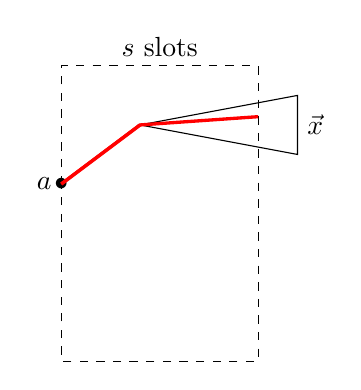
\begin{tikzpicture}[yscale=1.5]
\node at (0,0) [left] {$a$};
\node at (0,0) {$\bullet$};
%
\draw (0,0) -- (1, 0.5) coordinate(x);
%
\draw (x) -- ++(2,  0.25) -- ++(0, -0.5) node[pos=0.5,right]{$\vec{x}$} -- cycle;
%
\draw [dashed]
     (0,0)
  -- ++(0, 1)
  -- ++(2.5, 0) node[pos=0.5,above]{$s$ slots}
  -- ++(0, -2.5)
  -- ++(-2.5, 0)
  -- cycle;
%
\onslide<1>{
  \draw [red, very thick] (0,0) -- (1, 0.5) -- ++(1.5,0.07);
}
\onslide<2>{
  \draw [red, very thick] (0,0) -- (1, 0.5);
}
\end{tikzpicture}
\end{center}
\end{alertblock}

\end{frame}

%%%%%%%%%%%%%%%%%%%%%%%%%%%%%%%%%%%%%%%%%%%%%%%%%%%%%%%%%%%%%%%%%%%%%%%%%%%%%%%%

\begin{frame}{Prefix selection}

\begin{alertblock}{Step 2: Adopt common prefix (special case)}
\begin{center}
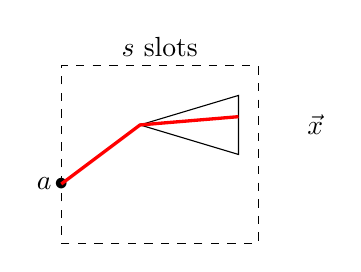
\begin{tikzpicture}[yscale=1.5]
\node at (0,0) [left] {$a$};
\node at (0,0) {$\bullet$};
%
\draw (0,0) -- (1, 0.5) coordinate(x);
%
\draw (x) -- ++(1.25,  0.25) -- ++(0, -0.5) node[pos=0.5,right=0.75cm]{$\vec{x}$} -- cycle;
%
\draw [dashed]
     (0,0)
  -- ++(0, 1)
  -- ++(2.5, 0) node[pos=0.5,above]{$s$ slots}
  -- ++(0, -1.5)
  -- ++(-2.5, 0)
  -- cycle;
%
\draw [red, very thick] (0,0) -- (1, 0.5) -- ++(1.25,0.07);
\end{tikzpicture}
\end{center}
\end{alertblock}

\pause

Smooth transition to longest chain rule.

\end{frame}

%%%%%%%%%%%%%%%%%%%%%%%%%%%%%%%%%%%%%%%%%%%%%%%%%%%%%%%%%%%%%%%%%%%%%%%%%%%%%%%%

\begin{frame}{Maximum rollback}

\begin{enumerate}

\item Ouroboros Praos assumes all nodes are online all the time

\item Imposes a maximum rollback of $k$ blocks

\item This is fine (Praos analysis tells us honest nodes won't diverge by more than $k$ blocks) \dots

\pause

\item \dots unless we are eclipsed by a malicious node and we adopt more than
$k$ of their blocks (reasonably long time)

\end{enumerate}

\end{frame}

%%%%%%%%%%%%%%%%%%%%%%%%%%%%%%%%%%%%%%%%%%%%%%%%%%%%%%%%%%%%%%%%%%%%%%%%%%%%%%%%

\begin{frame}{Maximum rollback}

\begin{enumerate}

\item Ouroboros Genesis drops the ``always online'' assumption \dots \pause

\item \dots as well as the maximum rollback \dots \pause

\item \dots but we don't want to do that

\end{enumerate}

\end{frame}

%%%%%%%%%%%%%%%%%%%%%%%%%%%%%%%%%%%%%%%%%%%%%%%%%%%%%%%%%%%%%%%%%%%%%%%%%%%%%%%%

\begin{frame}{Maximum rollback}

\begin{enumerate}

\item Genesis analysis tells us we do not need to roll back more than $k$
\emph{when we are up to date} (just like Praos)

\item When we are behind, prefix selection \emph{will always pick the honest
chain} at every intersection \dots \pause \textbf{provided it can see it}

\pause

\item Not a fundamentally new problem, difference in \emph{degree} only: when we are online, being eclipsed temporarily is fine.

\item But if we are behind, being eclipsed even for a very short amount can be disastrous: adversary can feed us $k$ blocks from their chain, we adopt them,
and are now stuck.

\pause

\item Solution: make sure to connect to a large number of upstream peers
(probably randomly chosen), and refuse to make chain selection decisions if
that quota is not reached.

\end{enumerate}

\end{frame}

%%%%%%%%%%%%%%%%%%%%%%%%%%%%%%%%%%%%%%%%%%%%%%%%%%%%%%%%%%%%%%%%%%%%%%%%%%%%%%%%

\begin{frame}{Being ``up to date''}

\begin{alertblock}{Recovering ``alert'' status}
When prefix selection can see all available chains to their tip, and we have
selected and adopted the best one, the node is up to date.
\end{alertblock}

\pause

When not up to date:

\begin{itemize}

\item Insist on quota of peers before chain selection

\item Do not produce blocks

\end{itemize}

\pause

When up to date:

\begin{itemize}

\item Danger of being eclipsed same as in Praos (very small, provided not too long)

\item Not entirely clear when to conclude we no longer up to date. Proposal from Frisby: ``as long as we stay connected to our current peers''.

\end{itemize}

\end{frame}

\end{document}
